\chapter{Appendix A} 
\label{appendix:anexo1}

The purpose of this appendix is to show more clustering analysis made for different vessels.

\section{Clustering analysis for vessel 1} % (fold)
\label{sub:clustering_vessel_1}
In Figure \ref{fig:elbow_method_1} is presented the value of the within sum of squares as function of the number of clusters, using the geographic coordinates data for vessel 1. As we can observe, three or six clusters seems to be a good number as the error is not decreasing much as the number of clusters increases. 


\begin{figure}[]
\centering
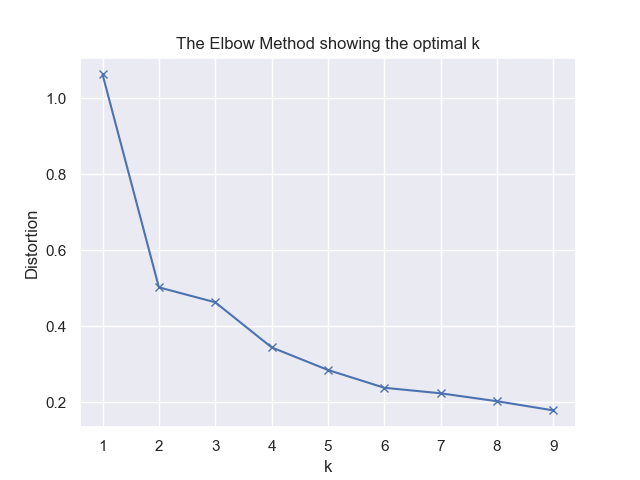
\includegraphics[width=0.8\linewidth]{Chapters/img/elbow_method1.png}
\caption{Sum of squared error as function of the number of clusters}
\label{fig:elbow_method_1}
\end{figure}


The average value of the Silhouette coefficient for vessel 1 is as described in Table \ref{table:vessel1_silhouette} with three having good values.

\begin {table}[H]
\caption {The average value of the Silhouette coefficient for vessel 1}
\begin{center}
\begin{tabular}{c|c}
\textbf{Number of clusters} & \textbf{Average silhouette coefficient}  \\
\hline
2 & 0.6337 \\
3 & 0.6542 \\
4 & 0.5784 \\
5 & 0.5731 \\
6 & 0.5658 \\
7 & 0.5819 \\
8 & 0.598 \\
9 & 0.5657
\label{table:vessel1_silhouette}
\end{tabular}
\end{center}
\end {table}


Considering the two methods I chose three as the number of clusters for the vessel 1.

\section{Clustering analysis for vessel 3} % (fold)
\label{sub:clustering_vessel_3}
In Figure \ref{fig:elbow_method_3} is presented the value of the within sum of squares as function of the number of clusters, using the geographic coordinates data for vessel 3. As we can observe, five clusters seems to be a good number as the error is not decreasing much as the number of clusters increases. 


\begin{figure}[]
\centering
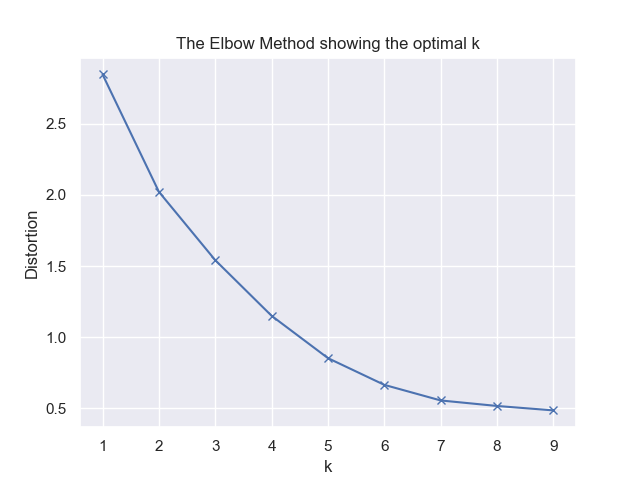
\includegraphics[width=0.8\linewidth]{Chapters/img/elbow_method3.png}
\caption{Sum of squared error as function of the number of clusters}
\label{fig:elbow_method_3}
\end{figure}


The average value of the Silhouette coefficient for vessel 3 is as described in Table \ref{table:vessel3_silhouette} with seven and nine having good values.

\begin {table}[H]
\caption {The average value of the Silhouette coefficient for vessel 3}
\begin{center}
\begin{tabular}{c|c}
\textbf{Number of clusters} & \textbf{Average silhouette coefficient}  \\
\hline
2 & 0.4751 \\
3 & 0.5629 \\
4 & 0.5616 \\
5 & 0.6063 \\
6 & 0.6532 \\
7 & 0.6629 \\
8 & 0.6607 \\
9 & 0.6647
\label{table:vessel3_silhouette}
\end{tabular}
\end{center}
\end {table}


Considering the two methods I chose seven as the number of clusters for the vessel 3.

\section{Clustering analysis for vessel 4} % (fold)
\label{sub:clustering_vessel_4}

In Figure \ref{fig:elbow_method_4} is presented the value of the within sum of squares as function of the number of clusters, using the geographic coordinates data for vessel 4. As we can observe, four clusters seems to be a good number as the error is not decreasing much as the number of clusters increases. 


\begin{figure}[]
\centering
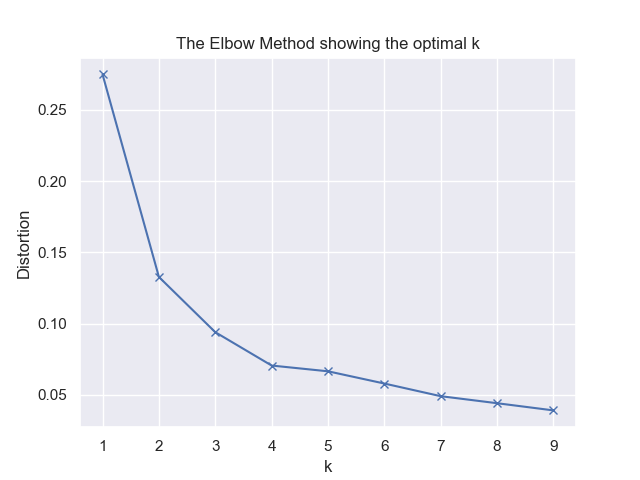
\includegraphics[width=0.8\linewidth]{Chapters/img/elbow_method4.png}
\caption{Sum of squared error as function of the number of clusters}
\label{fig:elbow_method_4}
\end{figure}


The average value of the Silhouette coefficient for vessel 4 is as described in Table \ref{table:vessel4_silhouette} with two having good values.

\begin {table}[H]
\caption {The average value of the Silhouette coefficient for vessel 4}
\begin{center}
\begin{tabular}{c|c}
\textbf{Number of clusters} & \textbf{Average silhouette coefficient}  \\
\hline
2 & 0.675 \\
3 & 0.5767 \\
4 & 0.5595 \\
5 & 0.5726 \\
6 & 0.5437 \\
7 & 0.5149 \\
8 & 0.5039 \\
9 & 0.4925 
\label{table:vessel4_silhouette}
\end{tabular}
\end{center}
\end {table}

Considering the two methods I chose tree as the number of clusters for the vessel 4.


\section{Clustering analysis for vessel 6} % (fold)
\label{sub:clustering_vessel_6}
In Figure \ref{fig:elbow_method_6} is presented the value of the within sum of squares as function of the number of clusters, using the geographic coordinates data for vessel 6. As we can observe, three clusters seems to be a good number as the error is not decreasing much as the number of clusters increases. 


\begin{figure}[]
\centering
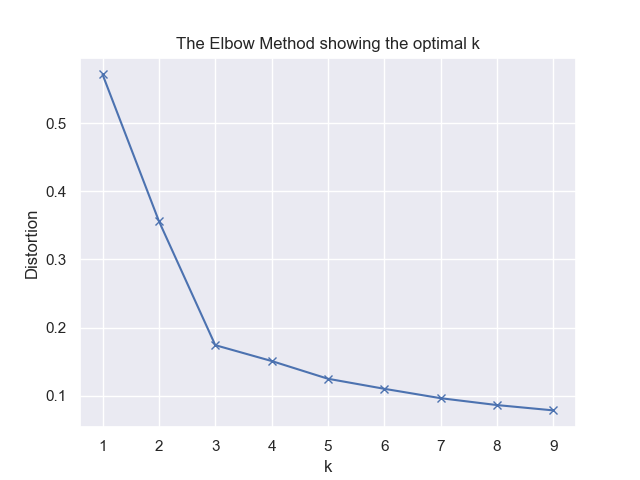
\includegraphics[width=0.8\linewidth]{Chapters/img/elbow_method6.png}
\caption{Sum of squared error as function of the number of clusters}
\label{fig:elbow_method_6}
\end{figure}


The average value of the Silhouette coefficient for vessel 6 is as described in Table \ref{table:vessel4_silhouette} with three having good values.

\begin {table}[H]
\caption {The average value of the Silhouette coefficient for vessel 6}
\begin{center}
\begin{tabular}{c|c}
\textbf{Number of clusters} & \textbf{Average silhouette coefficient}  \\
\hline
2 & 0.572 \\
3 & 0.684 \\
4 & 0.6531 \\
5 & 0.5638 \\
6 & 0.5115 \\
7 & 0.5154 \\
8 & 0.5202 \\
9 & 0.5083 
\label{table:vessel6_silhouette}
\end{tabular}
\end{center}
\end {table}


Considering the two methods I chose three as the number of clusters for the vessel 6.

\section{Clustering analysis for vessel 7} % (fold)
\label{sub:clustering_vessel_7}
In Figure \ref{fig:elbow_method_7} is presented the value of the within sum of squares as function of the number of clusters, using the geographic coordinates data for vessel 7. As we can observe, tree clusters seems to be a good number as the error is not decreasing much as the number of clusters increases. 


\begin{figure}[]
\centering
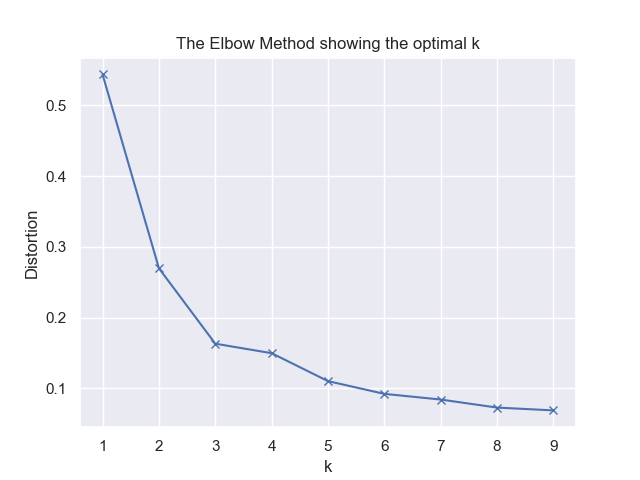
\includegraphics[width=0.8\linewidth]{Chapters/img/elbow_method7.png}
\caption{Sum of squared error as function of the number of clusters}
\label{fig:elbow_method_7}
\end{figure}


The average value of the Silhouette coefficient for vessel 7 is as described in Table \ref{table:vessel7_silhouette} with tree having good values.

\begin {table}[H]
\caption {The average value of the Silhouette coefficient for vessel 7}
\begin{center}
\begin{tabular}{c|c}
\textbf{Number of clusters} & \textbf{Average silhouette coefficient}  \\
\hline
2 & 0.6803 \\
3 & 0.7508 \\
4 & 0.7475 \\
5 & 0.6499 \\
6 & 0.5815 \\
7 & 0.5906 \\
8 & 0.5877 \\
9 & 0.5914 
\label{table:vessel7_silhouette}
\end{tabular}
\end{center}
\end {table}


Considering the two methods I chose tree as the number of clusters for the vessel 7.
